\documentclass[times, utf8, zavrsni]{fer}
\usepackage{booktabs}

\begin{document}

% TODO: Navedite broj rada.
\thesisnumber{1207}

% TODO: Navedite naslov rada.
\title{Detekcija kibernetičkih napada i zaštita vanjskih sustava u kontekstu mamaca za
operatora prijenosnog sustava}

% TODO: Navedite vaše ime i prezime.
\author{Filip Šimičević}

\maketitle

% Ispis stranice s napomenom o umetanju izvornika rada. Uklonite naredbu \izvornik ako želite izbaciti tu stranicu.
\izvornik

% Dodavanje zahvale ili prazne stranice. Ako ne želite dodati zahvalu, naredbu ostavite radi prazne stranice.
\zahvala{}

\tableofcontents

\chapter{Uvod}
Zbog napretka tehnologije pa tako i željom za pronalaženje boljih riješenja po pitanju održavanja električne mreže, operatori prijenosnih sustava se svakim danom razvijaju i koriste razne nove tehnologije i automatizacijske procese kako bi nam olakšali svakodnevni život. Međutim, time su uveli nove ranjivosti i rizike, posebno u području kibernetičke sigurnosti. Kibernetički napadi postali su značajna briga, prijeteći integritetu, dostupnosti i povjerljivosti osjetljivih informacija i kritične infrastrukture. Kako bi se osigurali od materijalne ili fizičke štete operatori prijenosnih sustava trebaju primjenjivati veće mjere zaštite i koristiti suvremene tehnologije koje pružaju optimalna riješenja za takve probleme. U ovom radu sam detaljno obradio zaštitu mamcima koji su samo jedan od temelja sigurnosti koji bi trebali biti implementirani u ovim sustavima. Implementacijom ovog modula, napadači mogu naići na naizgled ranjivu mašinu koja se lako podvija njihovm zahtjevima no u stvarnosti im u najmanju ruku trošimo vrijeme koje bi koristili za napad na pravi sustav. Također možemo prikupljati dragocjene podatke o samoj osobi koja stoji iza malicijoznih radnji.

\chapter{Operatori prijenosnih sustava}

\section{Definicija}
Uloge OPS-a na tržištu električne energije uključuju upravljanje sigurnošću elektroenergetskog sustava u stvarnom vremenu i koordinaciju ponude i potražnje za električnom energijom čime se izbjegavaju fluktuacije u frekvenciji ili prekidi u opskrbi. 
Svi OPS-ovi dužni su održavati stalnu (iz sekunde u sekundu) ravnotežu između opskrbe električnom energijom iz elektrana i potražnje potrošača, te također osigurati osiguranje rezervi koje će omogućiti iznenadne nepredviđene situacije. Većinom je državla vlasnik takvih institucija. [\cite{tso}] 

\section{PLC Sustavi}

PLC je programirljivi logički kontroler, tj. industrijsko računalo koje se sastoji od memorije, procesora, industrijskih ulaza i izlaza; ulazi nisu tipkovnica i miš, nego tipkala i sklopke, ili razne vrste pretvornika ili senzora.

PLC se najviše koristi kao osnovni dio upravljačkih automatskih sustava u industriji. Njegov program, odnosno algoritam, se može jednostavno mijenjati te je pogodan za brza rješenja i aplikacije. Dio je mnogobrojnih strojeva i procesa u industriji.
%\vspace{\baselineskip}

PLC je digitalno računalo, njegov program se izvršava ciklično i sastoji se od tri faze:
\begin{itemize}
\item{čitanje ulaznih varijabli}
\item{izvršavanje programskog koda}
\item{ispisivanje rezultata logičkih operacija na izlaze}
\end{itemize}

Program se pamti u unutrašnjoj memoriji uređaja i kad on ostane bez napajanja. Projektiran je za teške uvjete rada, otporan na vibracije, temperaturne promjene i električne smetnje. [\cite{plc2}]
\subsection{programski jezici}
Za kodiranje PLC-ova koristi se 5 programksih jezika:
\begin{itemize}
\item{ljestvičasta logika}
\item{dijagram funkcijskih blokova (FBD)}
\item{strukturirani tekst (ST)}
\item{popis uputa (IL)}
\item{sekvencijalna funkcionalna shema (SFC)}
\end{itemize} [ \cite{plc}]

\section{SCADA Sustavi}

\subsection{Arhitektura}
tipični SCADA sustav sastoji se od hijerarhije sljedećih komponenti:
\begin{itemize}
\item{pretvornika i aktuatora}
\item{RTU (eng. Remote Terminal Unit)}
\item{komunikacijske mreže}
\item{centralne stanice}
\end{itemize} [\cite{scada-arh}]
Ove komponente čine kontrolnu petlju nadzorne povratne sprege u SCADA sustavu.

\subsubsection{pretvornici i aktuatori}
Pretvornici i aktuatori predstavljaju početak lanca. Oni su električki ili mehanički vezani na proces koji promatramo. Zadaća pretvornika je praćenje vrijednosti tlaka, protoka, temperature, brzine... te da u analognom ili digitalnom obliku podatke o trenutačnom stanju mjerene veličine proslijede RTU-u. Aktuatori primaju informaciju od RTU-a te npr. zatvaraju ili otvaraju ventile.
[\cite{scada-thesis}]

\subsubsection{RTU (eng. Remote Terminal Unit)}
RTU-ovi su povezani s pretvornicima i aktuatorima i obično pohranjuju kontrolne parametre koje im senzori pošalju i izvršavaju programe koji izravno kontroliraju parametre električne energije. Stoga postoji stalna razmjena podataka i kontrola između RTU-ova, pretvornika i aktuatora koje tvore lokalnu povratnu kontrolnu petlju. RTU čuvaju prikupljene informacije u svojoj memoriji i čekaju zahtjev od MTU za prijenos podataka.
[\cite{scada-thesis}]

\subsubsection{komunikacijska mreža}
Komunikacijska mreža povezuje sve komponente ovog sustava i omogućuje im komunikaciju. Također omogućuje praćenje podataka u stvarnom vremenu.
[\cite{scada-thesis}]

\subsubsection{centralna stanica (MTU)}
MTU je glavna upravljačka jedinica koja sadrži stvarni SCADA softver, obično je povezana s mnogim RTU-ovim putem komunikacijskih kanala. MTU inicira sve komunikacije između RTU-a i sebe. Također je zadatak MTU-a da komunicira s drugim perifernim uređajima u objektu poput monitora, pisača, korporativne mreže i drugih informacijskih sustava. 

MTU provjerava RTU-ove u redovitim vremenskim intervalima kako bi pročitao podatke koje je prikupio RTU. Informacije o MTU prikazuju se na korisničkom sučelju kako bi se ljudskim operaterima omogućilo praćenje i upravljanje procesima pametne mreže. 

Operateri na MTU-u imaju mogućnost poništiti/promijeniti/nadjačati kritične radne parametre u bilo kojem dijelu SCADA mreže kada je to potrebno.

[\cite{scada-thesis}]

\subsection{Ranjvosti SCADA Sustava}
SCADA sustavi sami po sebi nisu građeni da zaštite podatke s kojima rukuju. Njihova zadaća je očitavanje senzora te određene akcije povratnom spregom ovisno o grani primjene. Potrebne su implementacije dodatnih zaštita kako bi se osigurali svi sigurnosni zahtjevi. 

Većina ovih sustava koriste Linux ili Windows operativni sustav koji imaju već globalno poznate ranjivosti koje napadači mogu iskoristiti. 
Još veći rizik se javlja ako su verzije operativnog sustava koji se koristi zastarjele.

Također se u ovakvim sustavim treba obratiti pozornost na protokole koji se koriste u mreži. Ako ti modeli ne sadržavaju adekvatnu kontrolu pristupa to sa sobom donosi skup problema koji potencionalno nisu ni riješivi sa zakrpama (engl. "patch").

Ovi izolirani sustavi se spajaju na globalnu mrežu kako bi operatorima omogućili spajanje i time dali uvid u komponente, njihova očitanja, upravljanje i sl. no to stvara i priliku za potencionalne napadače da dobiju pristup sistemu.
[\cite{scada-thesis}]

\section{Najčešće prijetnje}
Operatori prijenosnih sustava uz SCADA sustave koriste i razne druge koji omogućuju npr. povrzivanje zaposlenika unutar kompanije, isplaćivanje plaće, bilježenje radnog vremena. Oni također mogu biti kompromitirani i pružati vektor napada u sustav. Ako napadač dobije pristup na računalo nekog zaposlenika koji ima potrebne ovlasti za pristupanje nekom kritičnom dijelu sustava, cijeli taj blok postaje potencijonalno kompromitiran. 
ENISA has introduced the main categories of threats for 2020 [51] as follows: malware, web based/web application attacks, social engineering (phishing, spam), distributed denial of service, identity theft, data breach, insider threat, botnet, physical manipulation and damage, information leakage, ransomware, cyberwarfare/espionage and cryptojacking. [\cite{tso-vuln}]
\section{Zaštite koje se primjenjuju}
\begin{figure}[htb]
\centering
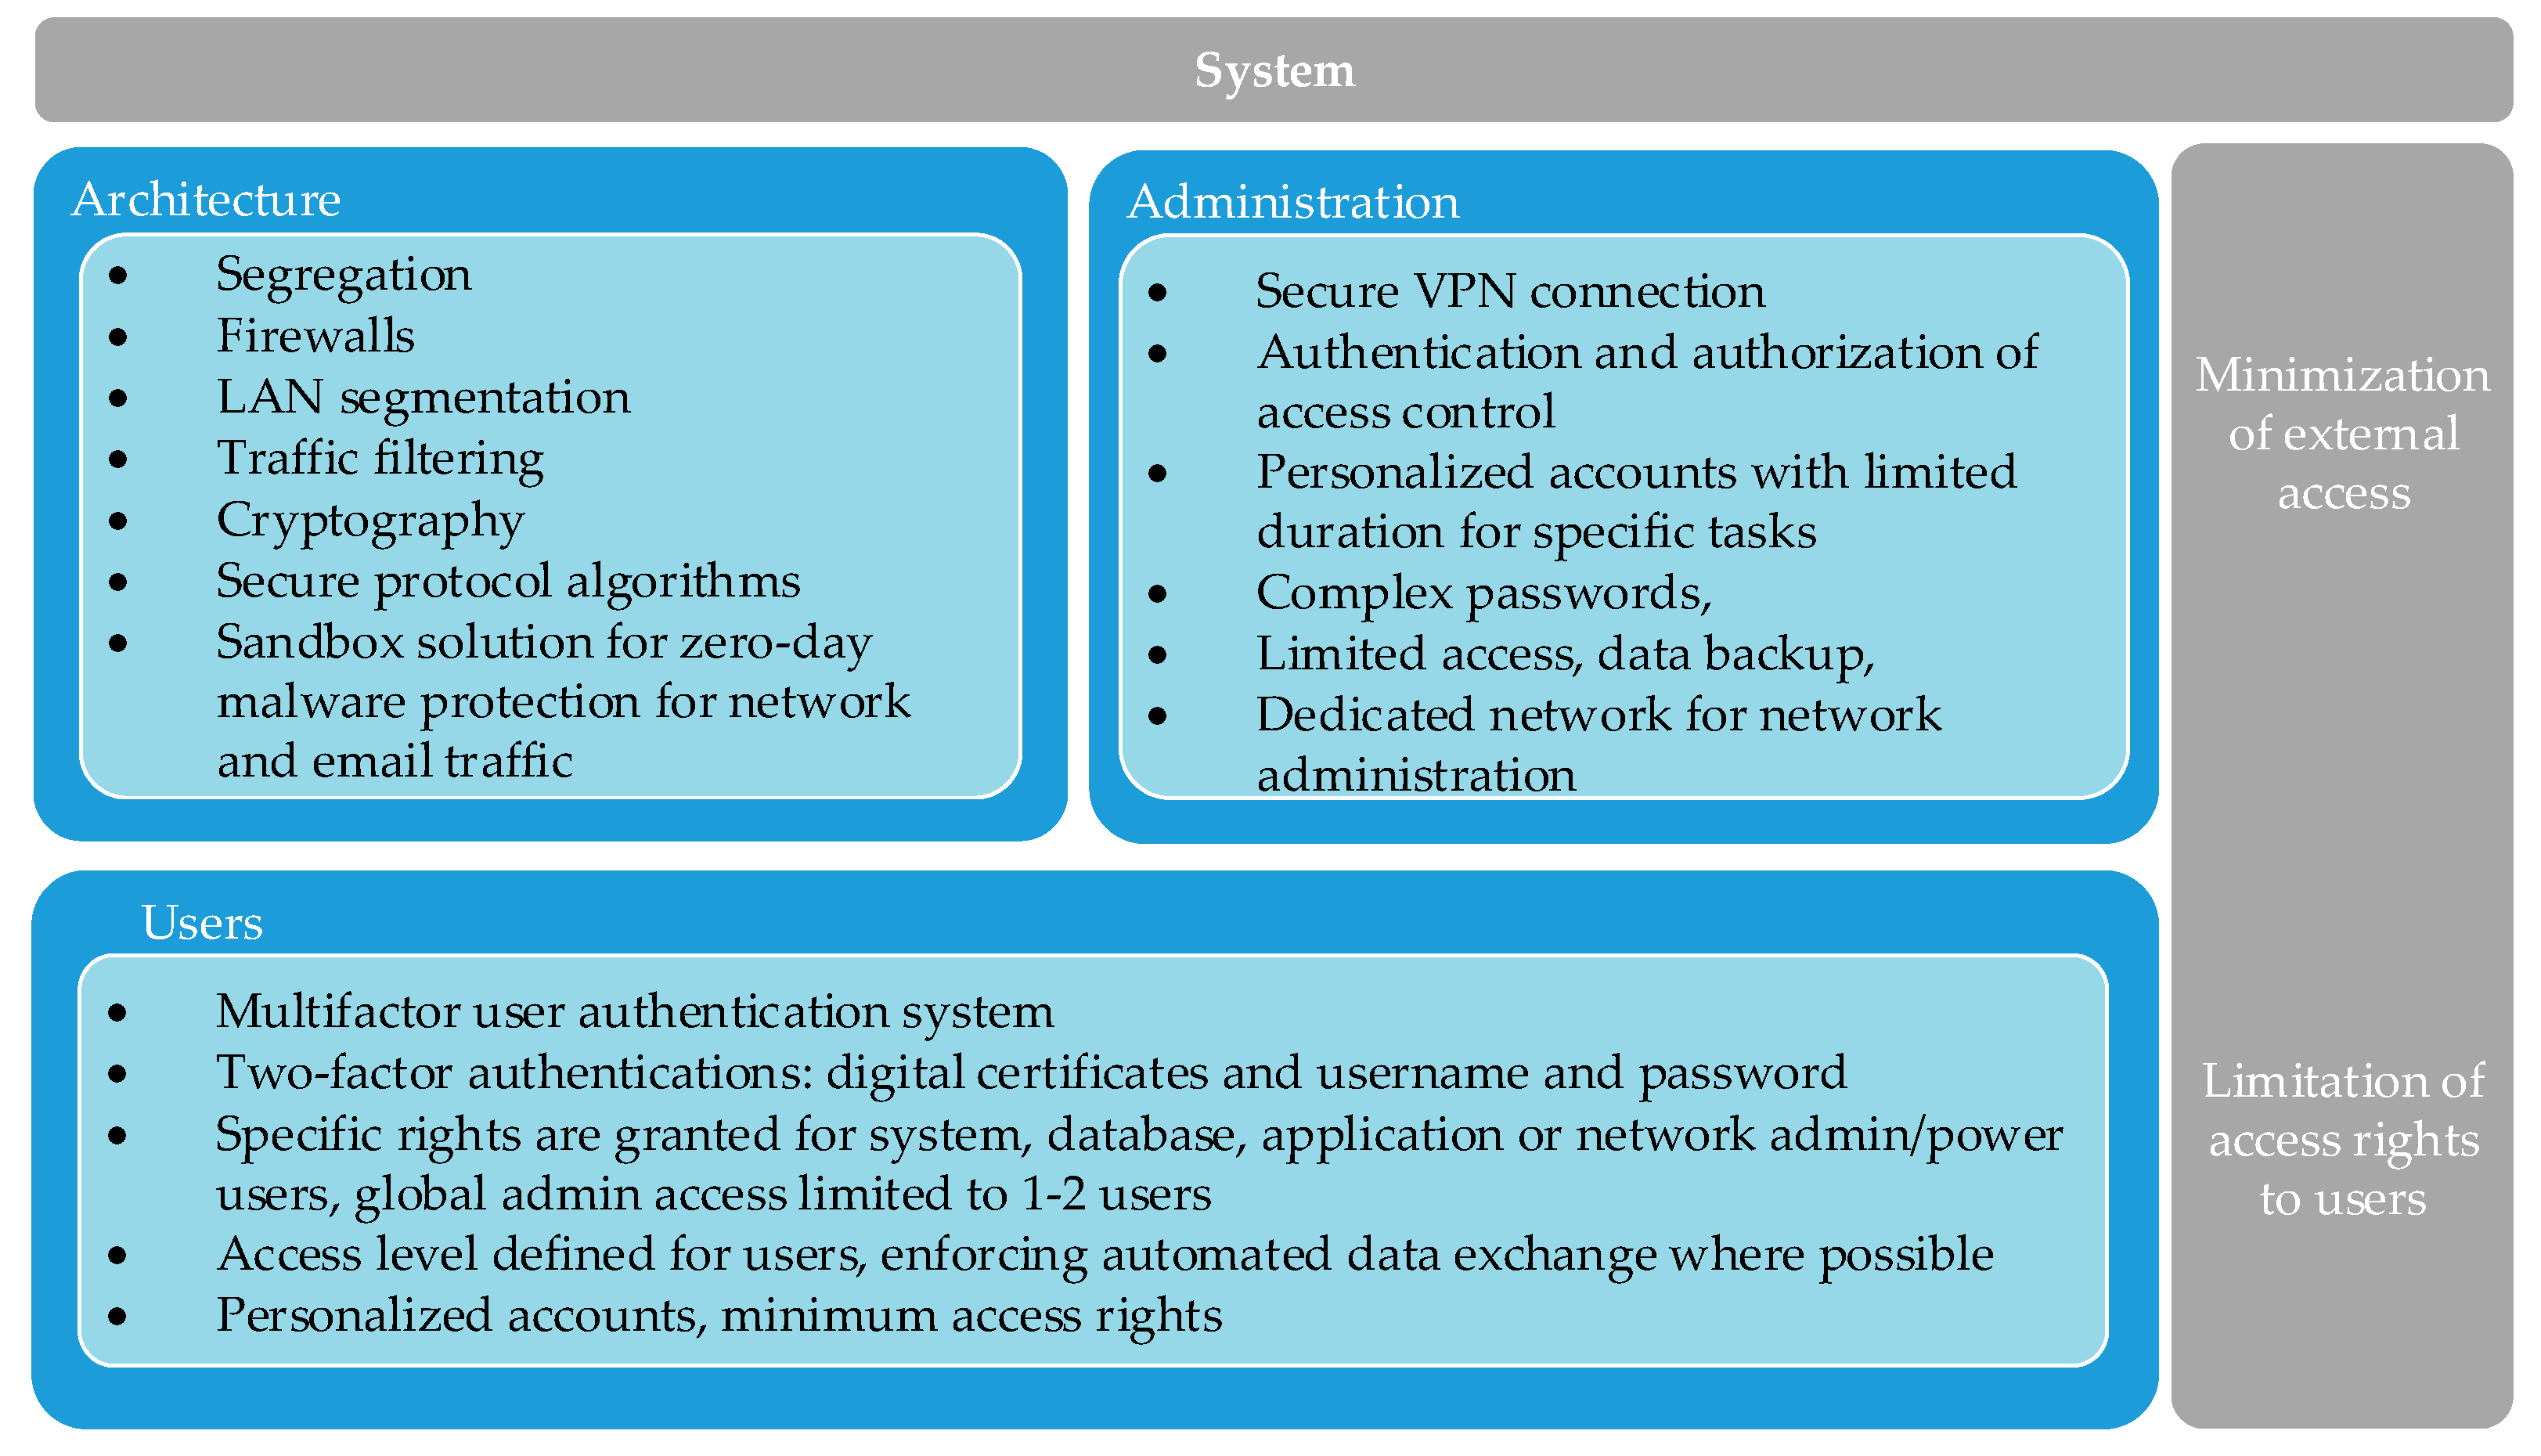
\includegraphics[width=14cm]{slike/Zastita-tso-sustava.png}
\caption{Zaštita OPS sustava  [\cite{tso-vuln}]}
\label{fig:Zastita-ops-sustava}
\end{figure}
Implementacija segregacije i vatrozida su među najčešćim mjerama zaštite zajedno s filtriranjem prometa i antivirusnim programima. Administrativni poslovi na važnim infrastrukturnim objektima obavljaju se putem računa koji nametaju određena ograničenja (ograničenje trajanja vremena, zaštita lozinkom, ograničenja pristupa). Uobičajeni pristup je implementacija višefaktorskog autentifikacije korisnika, ali također se koriste i specifična prava pristupa za korisnike koji obavljaju zadatke u kritičnim okruženjima (definicija različitih razina pristupa za različite vrste korisnika, personalizirani računi, minimalna prava za pristup). Korisnici trebaju biti motivirani i obučeni da održavaju potrebnu razinu opreza. [\cite{tso-vuln}] 

\section{OSINT nad Operatorom prijenosnih sustava}
\subsection{Definicija OSINTa}
OSINT je skraćenica za obavještajne informacije iz otvorenih izvora (eng. Open-Source Intelligence), što se odnosi na sve informacije koje se mogu legalno prikupiti iz besplatnih javnih izvora o pojedincu ili organizaciji. U praksi to obično znači informacije koje se nalaze na internetu, ali tehnički sve javne informacije spadaju u kategoriju OSINT-a bilo da se radi o knjigama ili izvještajima u javnoj biblioteci, člancima u medijima ili izjavama u saopštenju za javnost.
OSINT također uključuje informacije koje se mogu pronaći u različitim vrstama medija. Iako obično mislimo da je u pitanju samo tekst, informacije u slikama, video zapisima, webinarima, javnim govorima i konferencijama također spadaju pod taj pojam. 
[\cite{osint-def}]
\subsection{OSINT Alati}
\subsubsection{The Harvester}
\subsubsection{Shodan}
\subsubsection{Maltego}

\chapter{Docker}
\section{Odjeljak 3.1}

\chapter{Mamac (Honeypot)}
\section{Odjeljak 2.1}


\chapter{Imunes}
\section{Odjeljak 4.1}



\chapter{Zaključak}
Zaključak.

\bibliography{literatura}
\bibliographystyle{fer}
\begin{sazetak}
Sažetak na hrvatskom jeziku.

\kljucnerijeci{SCADA, Docker, OSINT}

\end{sazetak}

% TODO: Navedite naslov na engleskom jeziku.
\engtitle{Cyberattack detection and protection of external systems in the context of honeypots for transmission system operators}
\begin{abstract}
Abstract.

\keywords{SCADA, Docker, OSINT}

\end{abstract}

\end{document}
